\documentclass[10pt]{article}
\usepackage{amsmath}
\usepackage{geometry}
\usepackage{fancybox}
\usepackage{amsfonts}
\usepackage{amsbsy}
\usepackage{tikz}
\usepackage{listings}
\usepackage{amsthm}
\geometry{
a4paper,
total={170mm,257mm},
left=20mm,
top=10mm,
bottom=15mm
}
\usepackage{color}
\definecolor{codegreen}{rgb}{0,0.6,0}
\definecolor{codegray}{rgb}{0.5,0.5,0.5}
\definecolor{codepurple}{rgb}{0.58,0,0.82}
\definecolor{backcolour}{rgb}{0.95,0.95,0.92}

\linespread{1.3}

\title{CSC263H1 Assignment 6}
\author{Jiatao Xiang, Xu Wang, Huakun Shen}
\date{March 28th, 2019}

\begin{document}

\lstdefinestyle{mystyle}{
    backgroundcolor=\color{backcolour},   
    commentstyle=\color{codegreen},
    keywordstyle=\color{magenta},
    numberstyle=\tiny\color{codegray},
    stringstyle=\color{codepurple},
    basicstyle=\footnotesize,
    breakatwhitespace=false,         
    breaklines=true,                 
    captionpos=b,                    
    keepspaces=true,                 
    numbers=left,                    
    numbersep=5pt,                  
    showspaces=false,                
    showstringspaces=false,
    showtabs=false,                  
    tabsize=4
}
\lstset{style=mystyle}
\maketitle
\section*{Question 1}
\begin{itemize}
\item[a.]
\end{itemize}
\ovalbox{
\begin{tikzpicture}[level/.style={sibling distance=60mm/#1}]
\node [circle,draw, label=right:$1/12$] (z){$1$}
  child {node [circle,draw, label=right:$2/3$] (lz) {$6$}}
  child {node [circle,draw, label=right:$4/11$] (rz) {$4$}
    child {node [circle,draw, label=right:$5/8$] (rlz) {$5$}
    	child {node [circle, draw, label=right:$6/7$] (rllz) {$2$}}
		child[fill=none]{edge from parent[draw=none]}     
    }
  child {node [circle,draw, label=right:$9/10$] (rrz) {$7$}
	}
};
\end{tikzpicture}
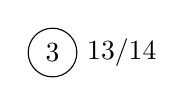
\begin{tikzpicture}[level/.style={sibling distance=60mm/#1}]
\node [circle,draw, label=right:$13/14$] (z){$3$};
\end{tikzpicture}
}
\begin{itemize}
\item[b.] Forward edge: 2, Back edge: 0, Cross edge: 5.
\item[c.] Use white-path theorem and parenthesis theorem.\\
To prove that it is possible to take all the courses
in a sequential order that satisfies all the prerequisite requirements, we have to prove that there are not two courses that are prerequisites of each other. \\
Suppose $u$ and $v$ are two nodes in $G$ that represent 2 courses, then $u$ is a prerequisite of $v$ if and only if $u.f>v.f$. So it is suffice to show that for every edge $(u,v)\in E$, $u.f>v.f$.
\begin{proof} To prove that $\forall$ edge $(u,v)\in E$, $u.f>v.f$.\\
\textbf{Case 1:} $(u, v)$ is a back edge\\
We know that, in the DFS forest above, there is no back edge, i.e. there is not cycle, so that there is not 2 courses being the prerequisites of each other.\\
\textbf{Case 2:} $(u,v)$ is a forward edge or tree edge\\
Then $v$ is a descendant of $u$. By parenthesis theorem, $u.d<v.d<v.f<u.f\Rightarrow u.f>v.f$\\
\textbf{Case 3:} $(u,v)$ is a cross edge\\
Then $u$ and $v$ are not descendants of one another, i.e. there is no prerequisite-relationship between $u$ and $v$, which means the order doesn't matter for these two courses. So we can make $u.f>v.f$ (i.e. take $u$ before $v$).\\
\end{proof}
\item[d.] $3\rightarrow 1\rightarrow 4\rightarrow 7\rightarrow 5\rightarrow 2\rightarrow 6$, in this ordering, each vertex's finish time is greater than the finish time of its next node.
\item[e.]
\end{itemize}
\ovalbox{
\begin{tikzpicture}[level/.style={sibling distance=60mm/#1}]
\node [circle,draw, label=right:$0$] (z){$3$}
  child {node [circle,draw, label=right:$1$] (lz) {$1$}
  	child {node [circle, draw, label=right:$2$] (llz) {$6$}}  
 	child {node [circle, draw, label=right:$2$] (lrz) {$4$}
 		child {node [circle, draw, label=right:$3$] (lrlz) {$5$}}
 		child {node [circle, draw, label=right:$3$] (lrrz) {$2$}}
 	}  
  }
  child {node [circle,draw, label=right:$1$] (rz) {$7$}
};
\end{tikzpicture}
}\\
Inside the node is the value of the node. Beside each node is the distance from node 3.




\section*{Question 2}
\textbf{Description:}\\
 First, we construct an adjacency list using all equality constraints. We also put all variables that not appeared in the equality constraints into the adjacency list. Since there are m constraints and n variables, constructing adjacency list totally takes $\mathcal{O}(m+n)$.\\
\begin{lstlisting}[language=Python]
def construct(x):
	# Construct an adjacency list using equality constraints all variables;
	make_adjacency_list()
	for each v in V:
		if color[v] is white
			# When each variable is explored, we create a field in it to store
			# the pointer points to the root.
			# Also give each root a distinct value.
			perform BFS and set v as the root
	for each x_i != x_j:
		if x_i.root == x_j.root:
			return NIL # contradiction!
	for each root of BFS tree:
		assign it with a unique number
		# each node in a tree has the same value with its root
\end{lstlisting}
BFS operation will change color[v] to black when it's fully explored and we loop over each line in the adjacency in order, therefore, after the for loop ends, every node in the list will be fully explored only once. This step takes $\mathcal{O}(m+n)$. At this stage, suppose there are k BFS trees produced, each of them was a connected graph where each node in it equal to each other. Then, we check inequality constraints, as long as we find a $x_i \neq x_j$ and they belongs to the same tree, then it's a contradiction and we return NIL. This step takes $\mathcal{O}(m+n)$. Otherwise, after this for loop ends, we assign proper number for each variable. This step takes $\mathcal{O}(m+n)$. Thus, the total cost is $\mathcal{O}(m+n)$.
\section*{Question 3}
Lemma: if the vertex is in the cycle, it must have at least two edges.\\
Intuitively, let u be a vertex that is in the cycle, then there must be an edge "out" of this vertex and an edge "into" this vertex, which shows that there must be at least two edges. This is stated in MST handout posted on course website.\\
Now prove by contradiction:\\
suppose there is a MST that contain $e_{max}$.\\
According to MST construction theorem, this would only happen when $e_{max}$ is the only path that connect one part of the graph to the other part, but every edge is in a cycle. Thus, contradiction! Since we have at least two edges for each node to connect to the rest of the graph, then we would choose the other edge instead of $e_{max}$, because the weight of the other edge must be less than or equal to the weight of $e_{max}$.\\
Thus, we conclude that there is no MST contain $e_{max}$.

\end{document}
